\subsection{Τρόπος Λειτουργίας}\label{subsec:visionDefinition}
Η όραση αποτελεί μία από τις βασικές αισθήσεις του ανθρώπου. Η αίσθηση αυτή βασίζεται στη λειτουργία του ματιού, το οποίο αποτελεί το αισθητήριο όργανο και στο εσωτερικό του οποίου εισερχεται το φως, διαπερνώντας αρχικά το κερατωειδή χιτώνα και την κόρη και προσπίπτει, τελικά, στον αμφιβληστορειδή χιτώνα (\hyperref[fig:eye_anatomy]{\schema~\ref*{fig:eye_anatomy}}). Αυτό οδηγεί σε διέγερση των οπτικών νεύρων και τα οπτικά σήματα, που αποστέλλονται στον εγκέφαλο, μετατρέπονται σε εικόνα~\cite{nationaleyeinstitute_2022_how}\cite{anspaugh_2022_vision}.

\begin{figure}[!h]
  \centering
  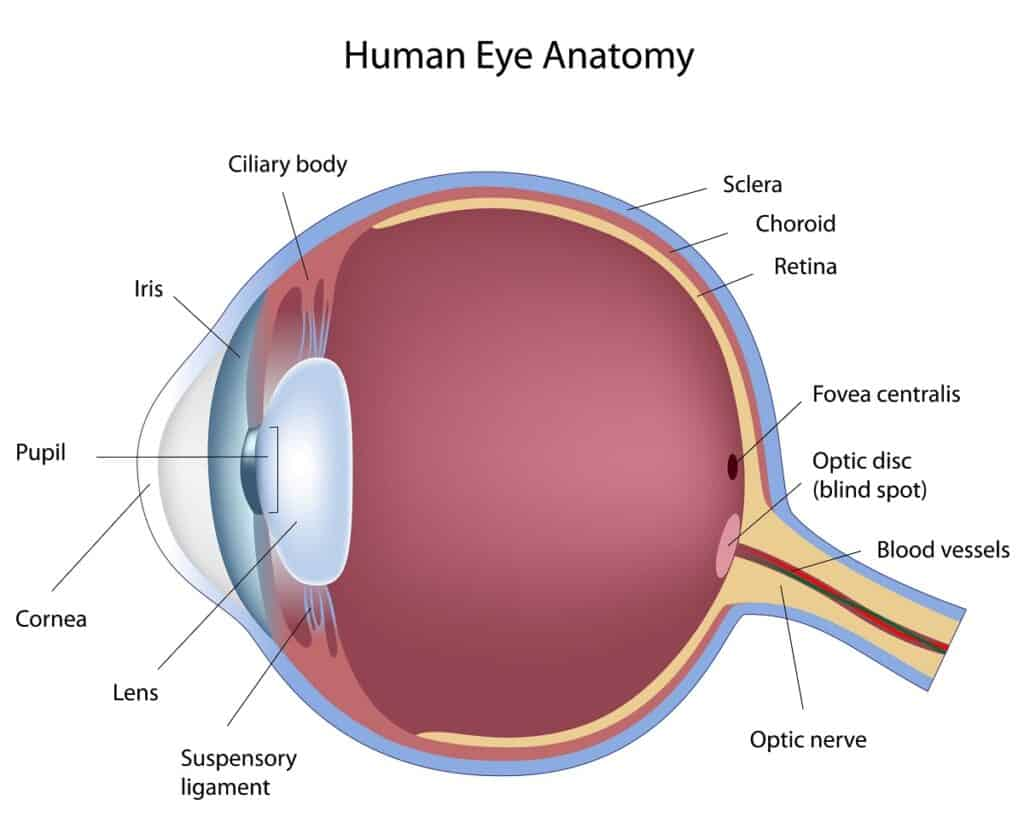
\includegraphics[width=90mm]{images/eye_anatomy.jpg}
  \caption{Η ανατομία του ματιού {\footnotesize(Πηγή: Dreamstime.com)}}\label{fig:eye_anatomy}
\end{figure}

\subsection{Απώλεια Όρασης: Κατηγοροποιήση και Αιτίες}\label{subsec:visionCauses}
Όταν η φυσιολογική λειτουργία του αισθητήριου οργάνου διαταραχθεί, τότε το άτομο έρχεται αντιμέτωπο με κάποιο τύπο προβλήματος όρασης. Με βάση τον Παγκόσμιο Οργανισμό Υγείας (Π.Ο.Υ.), τα άτομα αυτά κατηγοροποιούνται σε 6 κατηγορίες (Κατηγορία 0 έως Κατηγορία 5), ανάλογα την οπτική τους οξύτητα, δηλαδή της ικανότητάς του να διακρίνουν σχήματα και λεπτομέρειες από κάποια δεδομένη μακρυμένη απόσταση:
\begin{itemize}
    \item Στην κατηγορία 0 ανήκουν άτομα με με πλήρως ή σχεδόν πλήρως λειτουργική όραση
    \item Στην κατηγορία 1 και 2 ανήκουν άτομα που έχουν υποστεί μερική απώλεια της όρασής τους
    \item Τέλος, στις κατηγορίες 3, 4 και 5 εντάσσονται τα άτομα με σχεδόν πλήρη ή πλήρη απώλεια όρασης
\end{itemize}
Αντιθέτως, για κοντινές αποστάσεις, τα άτομα με προβλήματα όρασης εντάσσονται σε μία μόνο κατηγορία~\cite{worldhealthorganization_2019_world}.

Οι κυριότερες αιτίες, οι οποίες προκαλούν προβλήματα όρασης, απότελουν:
\begin{itemize}
    \item τα διαθλαστικά σφάλαματα
    \item ο καταράκτης
    \item η διαβητική αμφιβληστροειδοπάθεια
    \item το γλαύκωμα
    \item η ηλικιακή εκφύλιση της ωχράς κηλίδας
\end{itemize}
Από τα ανωτέρω, η κυριότερη αίτια πλήρης απώλειας όρασης σε άτομα ηλικίας 50 ετών και άνω αποτελεί ο καταράκτης, σε ποσοστό 46\% των ατόμων που υπέστησαν πλήρη απώλεια όρασης το 2020. Αντιθέτως, για την ίδια ηλικία ομάδα, η οποία αντιμέτωπιζε μερική απώλεια όρασης, κύριες αιτίες αποτελούν τα υποδιορθωμένα διαθλαστικά σφάλματα και ο καταράκτης, σε ποσοστό 30\% το καθένα για το ίδιο έτος~\cite{adelson_2021_causes}.

\subsection{Απώλεια Όρασης: Αντίκτυπος}\label{subsec:visionImpact}
Η απώλεια όρασης έχει ιδιαίτερο αντίκτυπο στην προσωπική, κοινωνική και οικονομική ζωή του ατόμου, ανεξαρτήτου της ηλικίας του. Η εκπλήρωση απλών καθημερινών εργασιών μπορεί να αποδειχθεί ιδιαίτερα δύσκολη και χρόνοβορα, επειδυνώνοντας ιδαίτερα την ποιότητα ζωής του ατόμου~\cite{west_2002_how}\cite{khorraminejad_2016_the}, ακόμη και σε επίπεδο χαμηλότερο από αυτό ατόμων που αντιμετωπίζουν χρόνια νοσήματα~\cite{langelaan_2007_impact}.



Η εμφάνιση προβλημάτων όρασης σε αρκετά νεαρή ηλικία μπορεί να επηρέασει αισθητά την ανάπτυξη ικανοτήτων όπως είναι η κινητήρια και η γνωστική του ικανότητα και η κοινωνική του καλλιέργεια~\cite{worldhealthorganization_2023_blindness}. Αντιθέτως, στην ενήλικη ζωή του, μπορεί να δυσκολέψει την εύρεση εργασίας και να επηρεάσει την ψυχική του υγεία, προκαλώντας μέχρι και άγχος και κατάθλιψη~\cite{khorraminejad_2016_the}. Τέλος, σε άτομα άρκετα μεγάλης ηλικίας, η απώλεια όρασης μπορεί να δυσχεράνει βασικές λειτουργίες, όπως είναι το περπατήμα με εγγενές κίνδυνο την πτώση και τον τραυματισμό~\cite{worldhealthorganization_2023_blindness}.

\subsection{Απώλεια Όρασης: Λύσεις}\label{subsec:visionSolutions}
Πλήθος λύσεων είναι διαθέσιμες στο μέσο άνθρωπο, οι οποίες στοχεύουν στην προτροπή της απώλειας της όρασης ή στην επιδιόρθωση αυτής. Σε απλές περιπττώσεις, όπως είναι η μυωπία, πρεσβυωπία, κ.λ.π., το πρόβλημα μπορεί να επιλύεται με χρήση διορθωτικών φακών ή εγχείρηση στο αισθητήριο όργανο~\cite{worldhealthorganization_2023_blindness}. Επίσης, για άτομα που δεν μπορούν επιδιορθώσουν το πρόβλημα όρασής του, έχουν αναπτυχθεί συσκευές και τεχνολογίες, οι οποίες συνεχώς εξελίσσονται και έχουν ως σκοπό την εξυπηρέτηση του ατόμου σε διάφορες πτυχές της καθημερινότητάς του. Επί δεκαετείες, το μπαστούνι αποτελεί μια αρκετά διαδεμένη συσκευή, που βοηθά ένα άτομο να αναγνωρίζει εμπόδια, καθώς περιηγείται σε έναν χώρο. Σε συνδυασμό με την απτική πλακόστρωση (\hyperref[fig:tactile_paving]{\schema~\ref*{fig:tactile_paving}}), το άτομο μπορεί να περιηγηθεί σε δημοσίο χώρο, όντας συνεχώς ενήμερος για την ύπαρξη εμποδίων, όπως δρόμοι, διάβαση πεζών, γραμμές τραμ, στη διαδρομή του, ανάλογα με το μοτίβο των πλακών του πεζοδρομίου~\cite{mashiata_2022_towards}.
\begin{figure}[!h]
  \centering
  \includegraphics[width=60mm]{images/tactile-paving.jpg}
  \caption{Απτική πλακόστρωση {\footnotesize(Πηγή: Vecteezy.com)}}\label{fig:tactile_paving}
\end{figure}\\
Ευρέως διαδεδομένη είναι και η χρήση σκύλων-βοηθών, οι οποίοι είναι ειδικά εκπαιδευμένοι σχετικά με την αναπηρία του ιδιοκτήτη τους με σκοπό να τους εξυπηρετήσουν στις ιδιαίτερες ανάγκες που μποροί να έχουν. Στην περίπτωση των ατόμων με πρβλήματα όρασης, σκοπός τους είναι να κατευθήνουν τον ιδιοκτήτης τους στο προορισμό τους, ειδοποιώντας τον για πιθανά εμπόδια~\cite{illinoisuniversitylibrary_2013_libguides}. Τέλος, αναπτύχθηκε το σύστημα γραφής Braille, ώστε να είναι εφικτή η ανάγνωση κειμένων με τη βοήθεια της αφής.

Στη σύγχρονή εποχή, όλο και περισσότερες συσκευές κατασκευάζονται λαμβάνοντας προκαταβολικά υπόψη τη δυνατότητα χρήσης αυτών από άτομα με περιορισμένη όραση. Οι κινητές συσκευές διαθέτουν λογισμικό screen reader (π.χ. TalkBack σε Android συσκεύες ή VoiceOver σε iOS συσκευές), διευκολύνοντας την πλοήγηση του χρήστη στις εφαρμογές του κινητού, καθώς πραγματοποιούν καταγραφή και αναγνώριση των κειμένων και των λειτουργιών, που βρίσκονται στη οθόνη τη δεδομένη χρονική στιγμή, και ο χρήστης, με συγκεκριμένες χειρονομίες, επιλέγει αν επιθυμεί την ανάγνωση κάποιο κειμένου με χρήση text-to-speech ή την πραγματοποίηση κάποιας ενέργειας~\cite{americanfoundationfortheblind_2019_screen}. Επιπλέον, η γλώσσα προγραμματισμού HTML δίνει τη δυνανότητα στους προγραμματιστές να κατασκευάσουν ιστοσελίδες, οι οποίες θα είναι προσβάσιμες από άτομα με περιορισμένη όραση, καθώς οι screen readers θα μπορούν να αναγνωρίζουν τμήματα της ιστοσελίδας, όπως επικεφαλίδες, υπερσύνδεσμοι, κουμπιά και το σκοπό που επιτελούν~\cite{w3schools_2020_html}.

Όσον αφορά την περιήγηση ατόμων σε ανοιχτούς ή κλειστούς χώρους, πληθώρα συσκευών έχουν κατασκευαστεί, οι οποίες βελτιώνουν ήδη υπάρχουσες ή προσφέρουν έναν εναλλακτικό τρόπο λειτουργίας και παροχής βοήθειας. Παραδείγματα τέτοιων συσκευών αποτελούν:
\begin{itemize}
  \item \textbf{biped}: Συσκευή, η οποία φοριέται γύρω από το λαιμό του χρήστη. Διαθέτει 3 κάμερες, που προσφέρουν πεδίο ορατότητας 170\textdegree, και ενσωματώνουν λογισμικό για τον εντοπισμό και αναγνώριση εμποδίων. Ο χρήστης προειδοποιείται για εμπόδια με μια ηχητική προειδοποίηση.~\cite{biped}
  \item \textbf{OrCam MyEye}: Φορητή συσκευή, η οποία προσφέρει τη δυνατότητα ανάγνωσης κειμένων, αναγνώρισης αντικειμένων, χρωμάτων και προσώπων.~\cite{ghebali_2023_orcam}
  \item \textbf{BlindSquare}: Εφαρμογή πλοήγησης, η οποία παρέχει αναλύτικες οδηγίες στο χρήστη, ώστε να κατευθυνθεί στο προόρισμο του, παρέχοντας παράλληλα πληροφορίες για το περιβάλλον του χρήστη και για σημεία ενδιαφέροντος.~\cite{blindsquare}
  \item \textbf{Be My Eyes}: Εφαρμογή, η οποία επιτρέπει σε χρήστες να έρθουν σε επικοινωνία με εθελοντές μέσω βιντεοκλήσης, με σκοπό να ζητήσουν βοήθεια.~\cite{a2019_be}
  \item \textbf{WeWALK}: Αποτελεί ένα εξάρτημα για μπαστούνια, το οποίο έχει τη δυνατότητα να εντοπίζει εμπόδια σε χαμηλό ύψος με χρήση υπερήχων και να ειδοποιεί το χρήστη με δονήσεις και ήχο.~\cite{wewalk}
  \item \textbf{Seeing AI}: Εφαρμογή της Microsoft, η οποία, με χρήση τεχνητής νοημοσύνης, παρέχει περιγραφές των αντικειμένων, χρωμάτων, ανθρώπων και κειμένων, τα οποία στοχεύει ο χρήστης με την κάμερα.~\cite{seeing}
\end{itemize}